\section{Sériový port}
Sériový port budíku umožňuje připojení jiného zařízení k rozhraní \acs{UART}
mikrokontroléru. Je použito signalizování na logických úrovních \acs{TTL}
(\SI{5}{\volt}) o rychlosti (\foreignlanguage{english}{baudrate})
\SI{9600}{\baud}, přenášeno je \num{8} datových bitů, bez parity a s jedním
stop bitem.

Použitý konektor umožňuje připojení redukcí firmy FTDI s modelovým číslem
\texttt{TTL-232R-5V-AJ}. Tato redukce se připojuje k počítači konektorem USB
typ A, obsahuje integrovaný obvod \texttt{FT232RQ} a její kabel je zakončen
audio konektorem Jack o průměru \SI{3,5}{\milli\meter} se třemi kontakty (TRS).
Zapojení konektoru je zobrazeno na obrázku~\vref{fig:UART jack pinout}.

\begin{figure}[htbp]
    \centering
    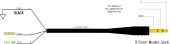
\includegraphics[width=\textwidth]{TTL-232R-5V-AJ-pinout.pdf}
    \caption{%
        Zapojení konektoru Jack USB--TTL UART převodníku
        \texttt{TTL-232R-5V-AJ}~\cite{TTL-232R}
    }
    \label{fig:UART jack pinout}
\end{figure}

Rozhraní \emph{není kompatibilní se standardem RS-232}, který používá napěťové
úrovně až \SI{\pm15}{\volt}.

V sérii se signály \texttt{Tx} a \texttt{Rx} jsou mezi konektorem Jack v zadním
panelu budíku a konektorem J5 (UART) na hlavní DPS zařazeny rezistory s odporem
\SI{1}{\kilo\ohm}. Tyto rezistory slouží jako ochrana před zkratem při
připojení nekompatibilního zařízení (například při připojení \texttt{Tx}
počítače na \texttt{Tx} budíku). Nejde ale o vhodnou ochranu proti připojení
příliš vysokého napětí na vstup \texttt{Rx}. Vstupní piny \acs{MCU} sice
obsahují ochranné diody, jejich specifikace ale nejsou zveřejněny a nelze je
považovat za vhodnou formu ochrany před přepětím.~\cite{dshATmega328}
